\documentclass{article}
\usepackage{biblatex}
\usepackage[utf8]{inputenc}
\usepackage[a4paper, total={5in, 11.5in}]{geometry}
\usepackage{hyperref}
\usepackage{caption}
\usepackage{graphicx}

\title{Truth teller's dice}
\author{Ruurd Bijlsma (S3860469) \\
Bharath Kumar Musuadhi Rajan (S4065476) \\
Jordi Timmermans (s3870758)
}

\begin{document}

\maketitle

\section*{Introduction}

We have implemented a modified version of the game ‘Liar’s dice’ using epistemic logic. We use the same rules as in the original game of 'Liar's dice' but simplify it by limiting the number of players to 3, the number of sides per dice to 2, and the number of dice to 1 making up for 8 possible worlds. The goal of the project is to explore and analyse different strategies that would emerge as a result of modelling the game using epistemic logic. We outline a few strategies later in this report. We run the game multiple times with varying strategies for each agent, to test which strategy works best. We display the logic lines along with its model visualization in a game simulation to better understand the game and explain why some strategy works better.

\begin{figure}[h]
    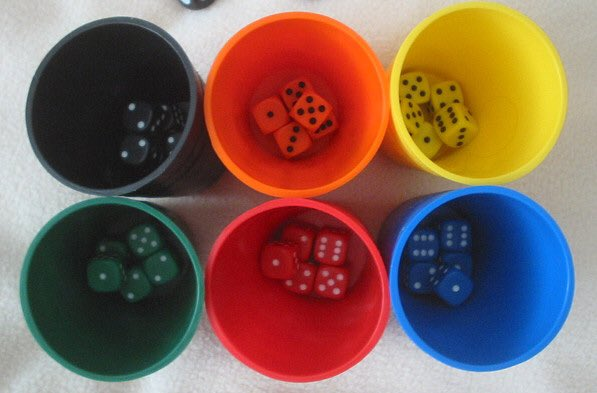
\includegraphics[width=0.9\textwidth]{img/Er3haXVXEAYrp0r.jpg}
    \centering
    \caption{Liar's Dice}
    \label{fig:liarsdice}
\end{figure}

\section*{Game description}
Liar's dice is a dice game for two or more players. Each player starts with a hand of dice, all players roll once, then the players take turns bidding what combination of dice the entire table has. During the players’ turn, they can either make a bid or challenge the previous bid. A bid is challenged when the player does not believe the previous bid is possible. When a challenge is made, the player calls out that the previously made bid is false and everyone must reveal their dice. If the challenge is correct (i.e., the previous bid is wrong), then the player who made the bid, loses one of their dice and the next round starts.

During Liar's dice a big part of the game is bluffing your bid, to not reveal information about your hand. In Truth teller's dice, there is no lying, meaning every bid must be something the agent considers possible, and an agent challenges a bid only if it knows that the previous bid is impossible.

\subsection*{Elements of the game} %ruurd
\begin{enumerate}
    \item 2 or more players
    \item N number of dice for each player
\end{enumerate}
\subsection*{Setup} %ruurd
At the start of each round every player rolls their dice and only looks at them their selves, no one else can see it.

\subsection*{Gameplay} %ruurd
The first agent makes a bid based on what it knows to be possible. A bid consists of a face value of the die, along with the total number of dice on the deck with that face value. For example, an agent can bid that there are two dice with the face value “1” on them. There are two possible bids that an agent can be make – 1) A bid that increases the quantity of dice retaining the number of pips (face value) of the previous bid, or 2) A bid that increases the number of pips retaining the current dice quantity. If one increases the pips, that player is able to call the number of dice starting from 1 again.

After each bid, the next agent decides if it must challenge the previous bid, or to continue with a new bid. If it knows that the previous bid is impossible (that there could not be that many dice of the same number of pips) based on its knowledge, then it challenges the bid; else the agent makes a new bid that it considers to be possible. 

When the agent decides to make a challenge, the round ends and all the agents reveals their dice. If the challenge is correct, the challenged player will lose a die, and a new round starts. If the challenge is not correct, meaning the previous bid was actually correct, then the challenger loses a die and the round restarts.

\subsection*{End of game} %ruurd
The game ends when only one agent is left with some dice, and this agent is the winner of the game.

\section*{Game implementation}
\subsection*{Initial configuration}
First an initial world list is created where all possible combinations of dice get listed. From these initial worlds, a connection matrix is set up where every element is the connection between two worlds. These elements contain who is not able to distinguish the two worlds. Besides this, two empty knowledge bases are initiated: one containing the logical knowledge of the agents and the other containing the bids.\\
After this the players get to roll their dice and look at their dice. The connection matrix gets updated based on the knowledge of the player. The output of the server when the game is initiated can be seen in figure \ref{fig:initc}
\begin{figure}[h!]
    \centering
    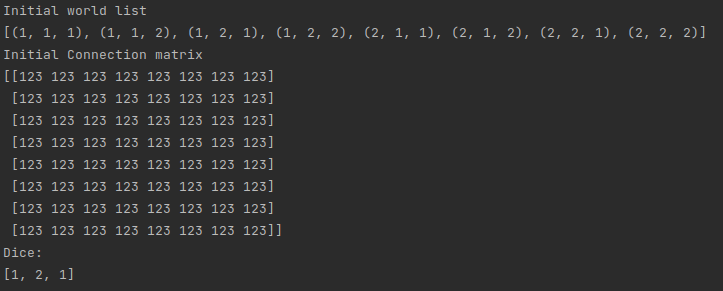
\includegraphics[width=\textwidth]{img/initialconfig.png}
    \caption{Initial configuration using 3 players, 1 die per player and 2 sides per die}
    \label{fig:initc}
\end{figure}
\subsection*{Rounds}
The first player either bids on the current dice, or a dice higher than the current dice. 
For every bid the player makes, the bid knowledge base as well as the logic knowledge base gets updated. When a player bids the maximum number of dice, all other players know what dice this player has because he did not lie. Therefore, the connection matrix gets updated. When the next player does not challenge the bid, all the other players also know what dice this player has, so the matrix gets updated yet again.\\
If a player loses a challenge or loses to a challenge, the losing player will lose a die and everything gets reinitiated.

An example of how a part of a round plays out can be seen in figure \ref{fig:halfaround}. the "quantities" refer to the highest bid per pip until now. So $[1\ 2]$ means someone bid 1 on 1 pip and 2 on 2 pips.
\begin{figure}[h!]
    \centering
    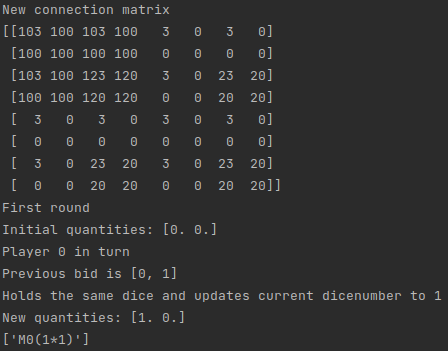
\includegraphics[width=.6\textwidth]{img/halfaround.png}
    \caption{Server showing the output after players looked at their dice and after player 0 announced a bit to update the number of dice with 1 pip to 1.}
    \label{fig:halfaround}
\end{figure}

\subsection*{Client-server connection} %ruurd
We implemented this project in two parts, the client as a web application, and the server as a Python program. This is because a user interface is easier to create in the web, and the logic part is easier to create in Python. The two parts communicate through WebSockets, the client connects to the server and sends a 'start game' event, the server then starts a game and saves it for this client, the server then sends information about the game through events to the client. The client can still request extra information or give commands through events, because an instance of the game is saved per client. 
\subsection*{Model visualization} %Ruurd
The model is visualized in the client using d3.js. The labels for the relations can be toggled, and it is possible to switch between Kripke models representing steps. This example model shows a game with two sided dice, 1 die per player, and three players. The labels for the worlds show what die each player has in that world. The unconnected worlds are worlds that are not possible anymore, no player considers them possible anymore. In this example, player A rolled 1, player B rolled 1, and player C rolled 2.
\begin{figure}[h]
    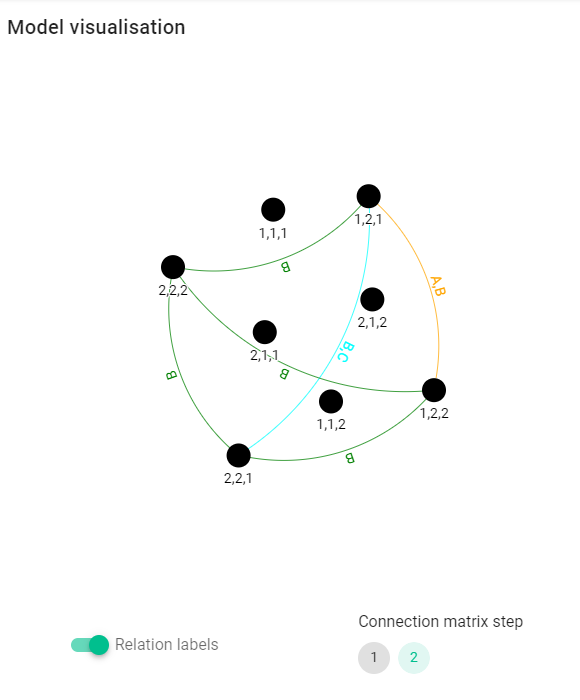
\includegraphics[width=0.8\textwidth]{img/visualization.png}
    \centering
    \caption{Model visualization after players have looked at their dice and one bid has been made.}
    \label{fig:liarsdice}
\end{figure}
\subsection*{Game visualization}% bharat

\section*{Logical modelling}
\subsection*{Example of a game}
\begin{enumerate}
    \item A game with 3 players, each with three 3-sided dice, will have the following atoms:\\
    (0*1), (1*1), (2*1), (3*1), ..., (9*1)\\
    (0*2), (1*2), (2*2), (3*2), ..., (9*2)\\
    (0*3), (1*3), (2*3), (3*3), ..., (9*3)\\
    \item In this situation there are 9 dice in total, and 3 sides per dice. In a Kripke model every world represents what each player has for dice. The number of worlds can be calculated by taking the combination with replacement $C^R(n,r)$ with n = number of sides per die, and r = number of dice. Then take the result of this to the power of $nPlayers$. So in our example, $C^R(3,3)^3 = 1000$, so there are 1000 possible worlds in this case.
    \item Before looking at their own dice each agent considers all these atoms possible ($M_a(0*1)$, ..., $M_c(9*3)$)
    \item Each agent gets to know what dice they rolled through a private announcement. After this announcement, each agent can eliminate some possibilities (if agent B has $[1, 1, 2]$ as dice, then $K_b \neg (9 * 3)$, $K_b \neg (8 * 3)$, $K_b \neg (7 * 3)$, $K_b \neg (9 * 1)$, $K_b \neg (9 * 2)$, $K_b \neg (8 * 2)$.). Some relations between worlds in the Kripke model could be cut after the announcement.
    \item The game starts when the first player makes a bid, for example, agent A announces he believes there are seven dice with a three on on it. This makes it common knowledge that agent A believes this is possible, so $CM_a(7 * 3)$.
    \item Because now every agent knows that agent a believes (7 * 3) is possible, every agent now also knows agent A has at least one die with a three (because there are only 9 dice in total, and agent A has three of them. $C \neg (0 * 3)$, it's now common knowledge that (0 * 3) is impossible. Agents that have a 3 themselves are able to eliminate more possibilities. 
    \item After agent A's bid, it's now agent B's turn. Agent B knows (7 * 3) is not possible ($K_b \neg (7 * 3)$ from (3)), so agent B must challenge the previous bid.
    \item After agent B's challenge, everyone reveals their dice and agent A will lose one die because he made a bid that turned out not to be true. This goes on until there is only one person with dice left.
\end{enumerate}
\subsection*{Model solver}%Explanation of the model solver here.
The model is solved by keeping track of a matrix that contains the connections for each word. Each element of the matrix initially contains connections for each player. Whenever a player gets more knowledge, the element might be adjusted because a player might be able to differentiate between two worlds. The real world will always contain all the reflexive connections because no one can differentiate between the real world and itself. 
\subsection*{Strategies} %ruurd
We will test multiple strategies for the agents. The strategies are used to decide which bid will be picked out of the possible legal bids, and when to make a challenge.
\subsubsection*{Challenging strategies}
\begin{enumerate}
    \item The strategy to challenge another player will be based on the number of dice in play and the dice the player holds. The probability of challenging is calculated by $100/(\#dice+1) * \#dice\ bid\ by\ previous\ player$ if the player holds a dice with the same number of pips as the bid had. If a player does not hold a dice with the same pips as the previous bid, the probability of challenging is calculated by $100/(\#Dice) * \#dice\ bid\ by\ previous\ player$. Here $\#dice$ means the number of dice in play.
\end{enumerate}
\subsubsection*{Bidding strategies}
\begin{enumerate}
    \item Bid one higher than the previous bid. Pick a legal move that is as close as possible to the previous bid.
    \item Random bid. Regardless of the previous bid, randomly pick a legal move.
    \item Bid as high as possible. Regardless of the previous bid, the agent always bids the highest possible legal move.
    \item Eliminate as few worlds as possible. Bid whichever legal move would eliminate the fewest possible worlds.
    \item Eliminate as many worlds as possible. Bid whichever legal move would eliminate the most possible worlds.
\end{enumerate}


\section*{Results}
% discuss winrate per strategy
% strategy advantage matrix
Will be added once we have them.
\section*{Conclusion and discussion}
% best winrate
% todo list
Will be added later.

%\bibliography{references}
\end{document}
